%\part{Aspectos Gerais}

\chapter[Referencial Teórico]{Referencial teórico}
	
	Este capítulo tem como objetivo servir como referencial teórico para todo o documento. As idéias discutidas neste capítulo são
	
\section{Processo de Contratação de Software na APF}
O Decreto n\c 2.271 de 1997 \cite{decreto_2271} dispõe sobre a contratação de serviços pela APF. Segundo o Decreto todos os produtos ou serviços que não apresentam relação direta com o propósito da instituição do governo federal devem ser tercerizados. O Decreto coloca como exemplo algumas atividades como por exemplo, conservação, limpeza, segurança, vigilância, transportes, informática, copeiragem, recepção, reprografia, telecomunicações são atividades livres para tercerização.
\\A licitação é um conjunto de processos administrativos de caráter formal para as compras de bens ou serviços nos governos federais, estaduais ou municipais. Segundo a Lei  n 8.666 de 1993, o governo brasileiro para garantir a isonomia (princípio geral do direito segundo o qual todos são iguais perante a lei) diz que para contratações de bens ou serviços deve-se dar prioridade para licitação \cite{Lei_1993}. A licitação pode ocorrer de quatro categorias: concorrência, tomada de preços, convite e pregão \cite{brazil_licitacoes_2010}.
\\Uma vez que uma empresa ganha a licitação para um serviço a empresa ganha o direito de contratação para prestar o serviço ao orgão contratante. Para ajudar no processo de contratação de empresas terceirizadas voltadas para a área de TI o TCU disponibiliza um Guia de boas práticas de contratações em soluções de TI \cite{guia_boas_praticas}. Segundo o guia a prática de contratação do serviço de desenvolvimento de um sistema de informação pode englobar elementos do tipo:
\begin{itemize}
\item Os softwares do sistema, devidamente documentados e com evidências de que foram testados;
\item As bases de dados do sistema, devidamente documentadas;
\item O sistema implantado no ambiente de produção do órgão;
\item A tecnologia do sistema transferida para a equipe do órgão, que deve ocorrer ao longo de todo o contrato;
\item As rotinas de produção do sistema, devidamente documentadas e implantadas no ambiente de produção do órgão;
\item As minutas dos normativos que legitimem os atos praticados por intermédio do sistema;
\item O sistema de indicadores de desempenho do sistema implantado, que pode incluir as atividades de coleta de dados para gerar os indicadores, fórmula de cálculo de cada indicador e forma de publicação dos indicadores. Citam-se, como exemplos, os indicadores de disponibilidade, de desempenho das transações e de satisfação dos usuários com o sistema de informação;
\item Os scripts necessários para prover os atendimentos relativos ao sistema por parte da equipe de atendimento aos usuários, devidamente implantados e documentados;
\item A capacitação dos diversos atores envolvidos com o sistema (e.g. equipe de suporte técnico do órgão, equipe de atendimento aos usuários, equipe da unidade gestora do sistema e usuários finais), que pode envolver treinamentos presenciais e a distância;
\item O serviço contínuo de suporte técnico ao sistema (e.g. atendimento aos chamados feitos pelo órgão junto à contratada sobre dúvidas e problemas relativos ao sistema);
\item O serviço contínuo de manutenção do sistema (e.g. implantação de manutenções corretivas e evolutivas).
\end{itemize} 


\section{Qualidade}
	O principal produto da engenharia de software é o software, contudo o que tem se vivenciado na realidade brasileira de computação é que o software que está sendo entregue é um software precário e de baixa qualidade. Por ser uma palavra abstrata, o conceito de qualidade é bem amplo, porém o termo qualidade normalmente está associado a uma medida relativa, essa qualidade pode ser entendida como "conformidade às especificações". Conceituando dessa forma, a não conformidade às especificação é igual a ausência de qualidade \cite{Paduelli}.
\\ A ISO 9126-1 proposta em 2001, também conhecida como Engenharia de Software - Qualidade do Produto, descreve o modelo de qualidade voltado para o produto de software como sendo composto por duas categorias como pode ser visto na Figura \ref{img:relacao_iso}. A primeira categoria está relacionada a qualidade interna e a qualidade externa do software. A segunda categoria se relaciona com a qualidade de uso do software \cite{_nbr_2016}
\graphicspath{{figuras/}}
\begin{figure}
\centering
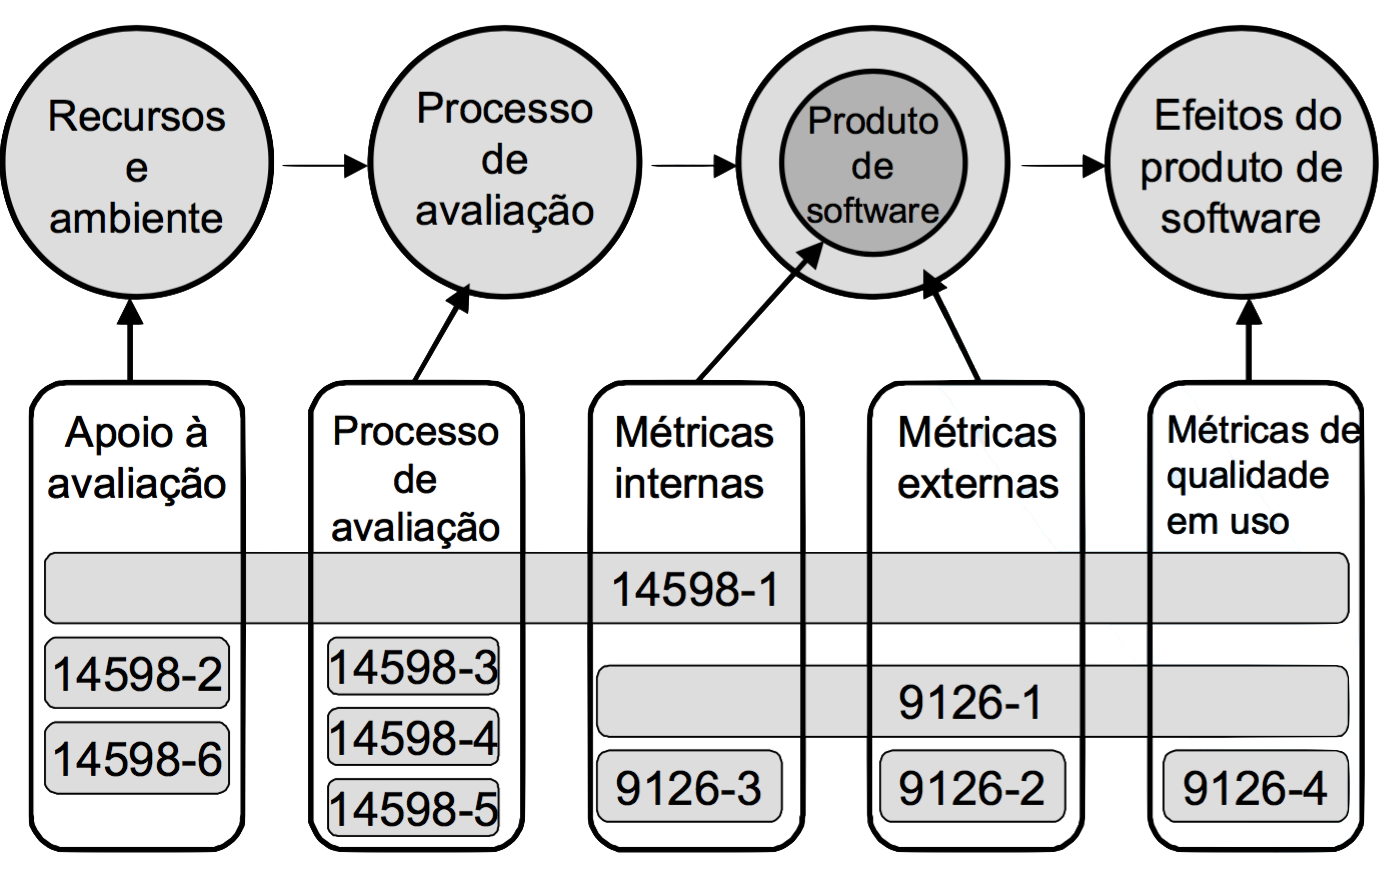
\includegraphics[scale=0.40]{ISO}
\caption{Relação entre as NBR ISO/IEC 9126 e NBR ISO/IEC 14598 .Fonte:\cite{_nbr_2016}}
\label{img:relacao_iso}
\end{figure}
\\ Sob o aspecto de modelo de qualidade,a ISO 9126 classifica a qualidade interna do produto como sendo o somatório das características do ponto de vista interno do software. Os principais produtos desta categoria são os de cunho intermediário, entre eles: relatórios de analise estática do código fonte, revisão dos documentos produzidos, entre outros. A qualidade externa por sua vez já apresenta o seu foco mais voltado para as relações externas do software, normalmente esta relacionado com a execução do código coletando suas métricas enquanto o software está em funcionamento. A Figura \ref{img:modelo_qualidade} apresenta a divisão proposta pela \cite{_nbr_2016} onde são categorizados seis aspectos de qualidade de software e suas subcaracterísticas, essas podem ser medidas por meio de métricas internas e externas. 
 \graphicspath{{figuras/}}
\begin{figure}
\centering
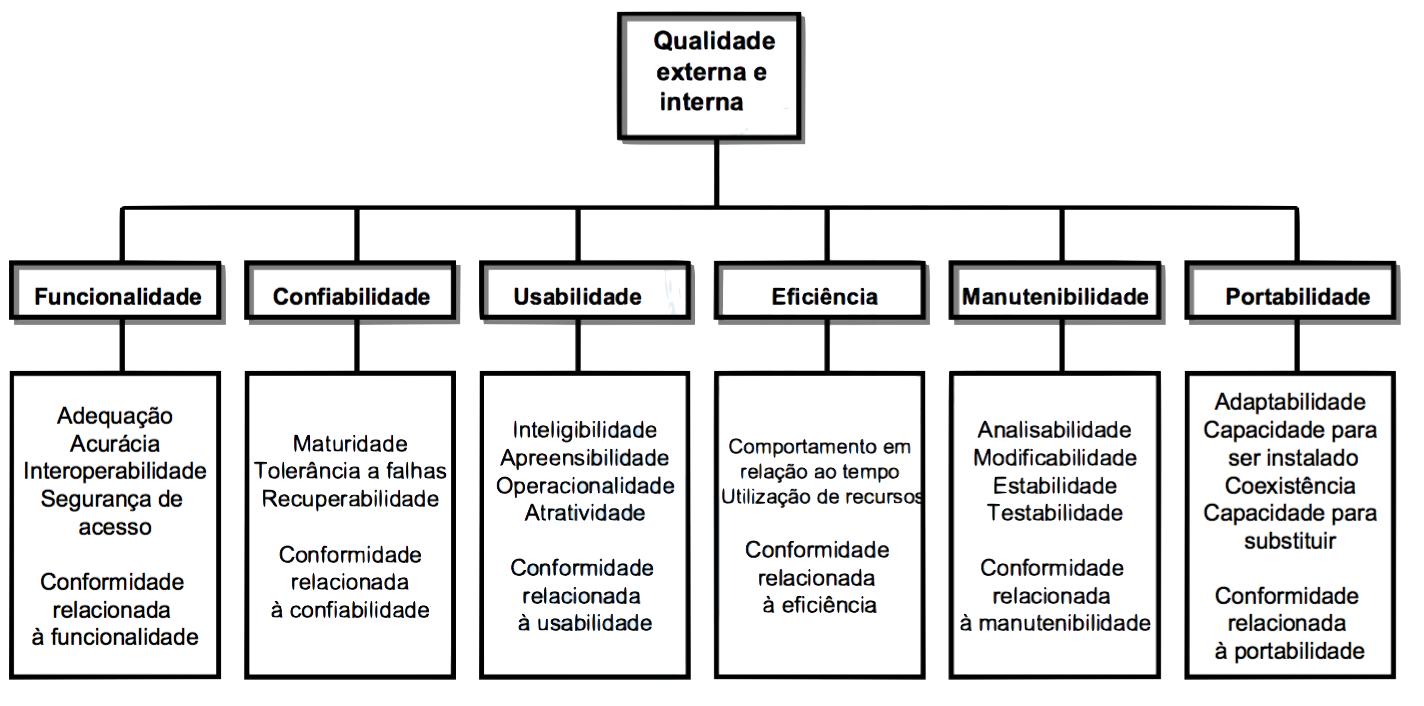
\includegraphics[scale=0.50]{Modelo_de_Qualidade}
\caption{Modelo de Qualidade para Qualidade Interna e Externa .Fonte:\cite{_nbr_2016}}
\label{img:modelo_qualidade}
\end{figure}
\\Segundo a ISO 9126 essas caracteristicas podem ser definidas como:
\begin{itemize}
\item \textbf{Funcionalidade}: Capacidade do produto de software de prover funções que atendam às necessidades explícitas e implícitas, quando o software estiver sendo utilizado sob condições especificadas.
\item \textbf{Confiabilidade}:Capacidade do produto de software de manter um nível de desempenho especificado, quando usado em condições especificadas.
\item \textbf{Usabilidade}: Capacidade do produto de software de ser compreendido, aprendido, operado e atraente ao usuário, quando usado sob condições especificadas.
\item \textbf{Eficiência}: Capacidade do produto de software de apresentar desempenho apropriado, relativo à quantidade de recursos usados, sob condições especificadas.
\item \textbf{Manutenibilidade}: Capacidade do produto de software de ser modificado. As modificações podem incluir correções, melhorias ou adaptações do software devido a mudanças no ambiente e nos seus requisitos ou especificações funcionais.
\item \textbf{Portabilidade}: Capacidade do produto de software de ser transferido de um ambiente para outro.
\end{itemize}
Em 2011 surgiu um conjunto de normas conhecidos como SQuaRE que traziam um framework aprimorado à atual norma vigente. Este framework tinha como objetivo avaliar o produto de qualidade de software.

\subsection{Norma SQuaRE}
O conjunto de normas SQuaRE (Requisitos e Avaliação de Qualidade de Sistema e Software) surgiu para substituir a ISO/IEC 9126. O objetivo destas normas é prover um framework que avalie a qualidade do produto de software \cite{luiza_yago}. ISO/IEC 25010 mantém as características de qualidade já definidas na ISO 9126 com alguns incrementos.

\begin{itemize}
\item O escopo dos modelos de qualidade foram extendidos para incluir sistemas computacionais e a qualidade em uso pelo ponto de vista do sistema
\item Segurança foi adicionada como característica, e não uma subcaracterística de funcionalidade.
\item Compatibilidade foi adicionada como característica.
\item A qualidade interna e externa foram combinadas como modelo de qualidade de produto.
\end{itemize}

A norma apresenta três guias de qualidade. O primeiro modelo é referente à Qualidade do Produto, o segundo da Qualidade em Uso e o último Qualidade de Dados.O modelo de Qualidade do Produto subdivide um sistema de software em oito categorias como mostra a imagem \ref{img:modelo_square}.
Assim como a ISO 9126, a ISO 25010 também apresenta categorias, estas categorias se assemelham às categorias da ISO 9126 a qual serviu como base para criação da norma SQuaRE, estas caracteristicas são:

\begin{itemize}
\item \textbf{Adequação Funcional}: nível que determina o quanto um produto ou sistema satisfazem as especificações providas pelo usuário.
\item \textbf{Eficiência de Performance}: performance relativa à quantidade de recursos usados em condições específicas.
\item \textbf{Compatibilidade}: o nível que um sistema ou produto pode compartilhar informaçõesc com outros produtos, sistemas ou componentes.
\item \textbf{Usabilidade}: O nível que um produto ou sistema pode ser usado por usuários específicos para atingir seus objetivos com efetividade, eficiência e satisfação em contexto específico de uso.
\item \textbf{Confiabilidade}: nível que um sistema, produto ou componente executa suas atividades em um contexto pré-determinado e específico para uso.
\item \textbf{Segurança}: nível no qual um sistema protege as informações e os dados de maneira que pessoas ou outros sistemas tenham acesso limitado de acordo com nível de autorização especifíco.
\item \textbf{Manutenibilidade}: nível de efetividade e eficiência com o qual um produto ou sistema pode ser modificado pelos sistemas mantenedores.
\item \textbf{Portabilidade}: Nível de efetividade e eficiência com o qual um sistema, produto ou componente pode ser transferido de um hardware, software ou ambiente de uso para outro.
\end{itemize}

\graphicspath{{figuras/}}
\begin{figure}
\centering
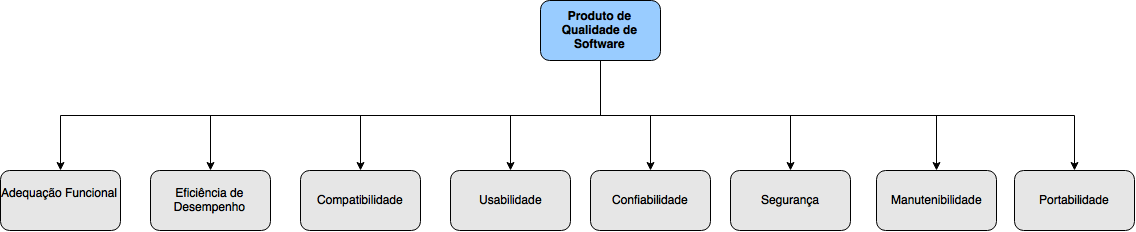
\includegraphics[scale=0.40]{SQuaRE}
\caption{Produto de Qualidade de Software.Fonte:\cite{Square}}
\label{img:modelo_square}
\end{figure}

Este trabalho tem seu desenvolvimento focado no modelo de Qualidade de Uso que apresenta características externas ao software e os resultados são coletados através de atributos estáticos \cite{Square}. O foco deste trabalho está em medir indicadores quanto à manutenabilidade do software. Essa característica está diretamente ligada ao processo de Manutenção do Software.  

\subsection{Manutenção de Software}
Segundo Sommervile \cite{sommervile} manutenção de software é o processo de alterar o sistema depois que ele foi publicado. As alterações feitas no software podem ser simples correções de erro, a até mudanças significativamente grandes que corrigem falhas arquiteturais, ou mesmo melhorias para acomodar novos requisitos.
\\Outra visão sobre manutenção de software é dada por Pressman \cite{pressman} em que o autor conceitua o termo como sendo a correção de defeitos, adaptação do software para atender uma mudança do ambiente e aperfeiçoar as funcionalidades para que atendam às necessidades dos usuários. Outra característica do processo de manutenção é a sua composição por um conjunto de sub processos, atividades e tarefas que podem ser utilizados durante a fase de manutenção para alterar um produto de software, contanto que seja mantido o seu funcionamento \cite{calazans_avaliacao_2005}.
\\Para Sommervile existem quatro categorias de manutenção:
\begin{itemize}
\item \textbf{Manutenção Corretiva}: seu objetivo está em identificar e remover falhas de software
\item \textbf{Manutenção Adaptativa}: provê modificações no software para alojar mudanças no ambiente externo. Nesta manutenção também está incluso o processo de migração para diferentes plataformas tanto de software quanto de hardware.
\item \textbf{Manutenção Perfectiva}: está manutenção é feito com o intuito de aperfeiçoar o software, além dos requisitos funcionais originais. Esta expansão dos requisitos traz consigo uma melhoria às funcionalidades até então implementadas ou um ganho de performance do sistema.
\item \textbf{Manutenção Preventiva}: implementada para permitir que seja mais simples a correção, adaptação ou melhoria do software.
\end{itemize}

O modelo da figura \ref{img:modelo_manutencao} apresenta as atividades propostas por Pfleeger para um processo de manutenção. Na figura percebe-se que o processo de acompanhamento da manutenção ocorre durante todo o processo. As atividades apresentadas no diagrama são:

\begin{itemize}
\item \textbf{Analise do Impacto da Mudanção de Software}: estima o impacto de uma determinada mudança. Nesta atividade determina-se o grau de mudança e o quanto está mudança impactará no resto do software. 
\item \textbf{Entendimento do Software a ser Alterado}: nesta atividade são analisados os códigos-fonte do software para entender a mudança e a integração do que deve ser alterado. Esta atividade depende muito do grau de manutenabilidade do software, uma vez que quanto mais manutenível mais fácil e rapido se dá o processo de analise do software.
\item \textbf{Implementação da Mudança}: incremento ou modificação do software. Está atividade é diretamente relacionada com o grau de adaptação do software, o quanto o software pode ser expandido ou comprimido. Essa característica de adaptabilidade é uma subcaracterística da Manutenabilidade de software apresentada pela norma Square. 
\item \textbf{Mudanças pelo Efeito Cascata}: Analise da propagação das mudanças ao longo do software. Essa atividade está intimamente relacionada com o indicador de coesão e acomplamento do software, este afere o quão amarrado estão as classes e os métodos do software.
\item \textbf{(Re)Teste do Software}: é a ultima atividade antes da entrega do software alterado. O software é testado novamente sob a perspectiva do novo requisito.
\end{itemize}

\graphicspath{{figuras/}}
\begin{figure}
\centering
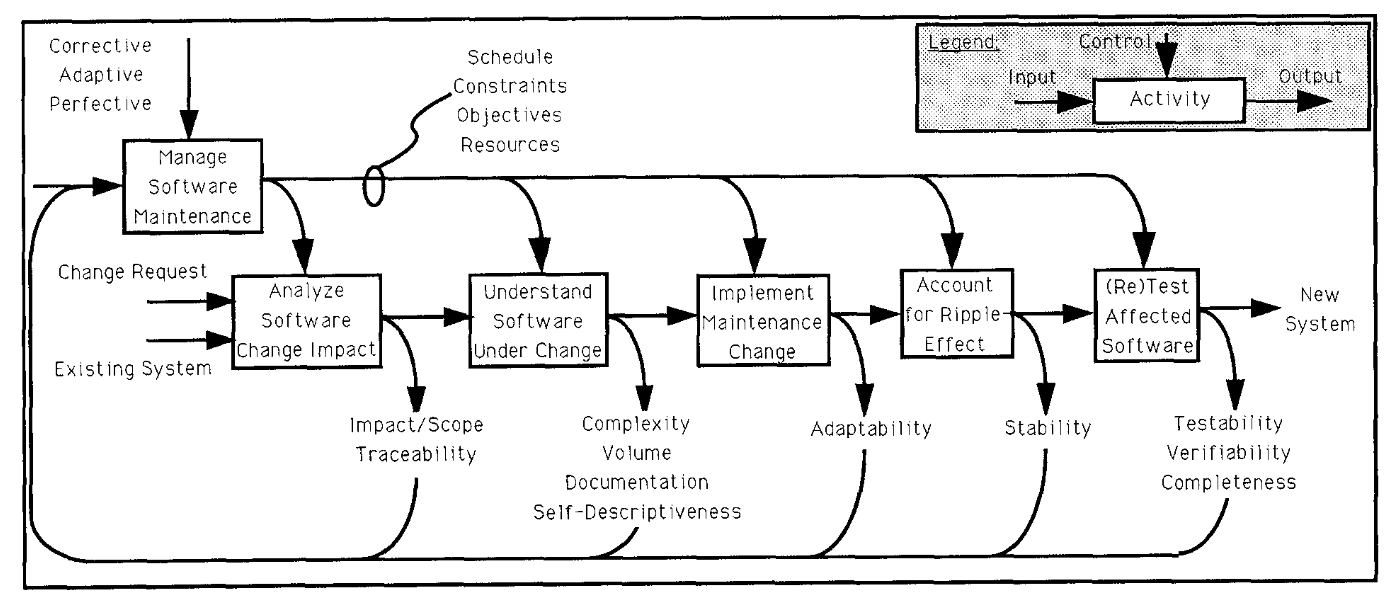
\includegraphics[scale=0.50]{Manutencao}
\caption{Diagrama das Atividades de Manutenção de Software.Fonte:\cite{pfleeger_framework_1990}}
\label{img:modelo_manutencao}
\end{figure}
Um estudo realizado por Kustyers e Heemstra \cite{kusters} mostram a dificuldade de atuais na manutenção de software em seis grandes organizações da Alemanha. Um dos resultados obtidos foi que existe um uma falta muito grande na percepção quanto ao tamanho e o custo das manutenções de software. Os autores relatam que os gastos com manutenção são altos e que das seis empresas apenas uma mantinha registrado os seus processos de manutenção e os usava para fazer um novo planejamento. 
\\Normalmente tem se como verdade de que a manutenção de software está unicamente ligada ao conserto de \textit{bugs}, entretanto estudos e \textit{surveys} ao longo dos anos comprovam que mais de 80\% do esforço gasto na manutenção é utilizado em ações não corretivas segundo Pigosky \cite{pigosky}. O autor também afirma que entre 40\% a 60\% do esforço de manutenção está em entender o software que será modificado.

\section{Métricas de Qualidade de Software}
Uma métrica é uma função que pode ser medida, e métrica de qualidade de software é uma funcão na cuja entrada é uma informação de software e cuja saida é um único valor numérico que pode ser interpretado como nível que é dado a um software \cite{karner}. Segundo \cite{pressman} métricas podem ser definidas como sendo um pequeno subconjunto de informações que tem informações úteis acerca do software.
Segundo Mills algumas características são inerentes a uma boa métrica, caracteristicas como, simplicidade,objetividade, fácil obtenção, validade, robustez, linearidade de escala. Diversos autores sugeriram conjunto de métricas que combinadas tratam de várias áreas de qualidade de software \cite{paulo_meirelles}.

\subsection{Suíte de Chidamber-Kemerer}
Este conjunto de métricas foi proposto por Shyam R. Chidamber e por Chris F. Kemerer em 1994 tem como objetivo avaliar aspectos de qualidade interna dos artefatos produzidos sob a visão de uma linguagem orientada a objetos \cite{chidamber}. A suíte apresenta as seguintes métricas:
\begin{itemize}

\item \textbf{WMC}: Em uma classe com \textit{n} métodos, a complexidade é dada como sendo a complexidade dos \textit{n} métodos. 
 \begin{equation}
WMC = \sum_{i=1}^{n}Ci
\end{equation}


Essa métrica serve como indicador para o nível geral da modularização. Quanto maior o valor mais complexas estão a classe ou poucas classes possuem um indíce de complexidade muito alto.

\item \textbf{DIT}: Tamanho do maior caminho entre a raiz da árvore de herança e a classe a qual está sendo analisada. Essa métrica permite ver o quanto uma mudança em uma determinada classe pode afetar todo o sistema.

\item \textbf{NOC}: Quantidade de classes que se utilizam da classe em analise, seja por herança ou implementação. Essa métrica junto com outras ajuda a determinar quais classes são primordiais para o funcionamento do sistema.

\item \textbf{CBO}: Está métrica é dada pela equação 2.2: 

\begin{equation}
CBO = \frac{NumberOfDependencies}{NumberOfClassInPackage}
\end{equation}
Uma dependência pode ser definida como o uso de um método ou variável de outra classe porém do mesmo pacote.

\item \textbf{RFC}: Número de métodos e construtores distintos que são chamados por uma classe. Está medida é muito utilizada para cobertura de testes, em que é pode ser constatado a necessidade ou não de uma modularização de uma classe.

\item \textbf{LCOM}: Sendo \textit{C} uma classe com \textit{n} métodos, seja \textit{In} o conjunto de variáveis de instância utilizadas pelo método \textit{n}, seja \textit{P} o conjunto tal que:
\begin{equation}
P = \{(Ii,Ij)|(Ii\bigcap Ij)= \o\}
\end{equation}
e \textit{Q} o conjunto tal que:
\begin{equation}
Q = \{(Ii,Ij)|(Ii\bigcap Ij)= \o\}
\end{equation}
então LCOM é definida como sendo:
\begin{equation}
LCOM = |P| - |Q| se |P|>|Q|
\end{equation}
ou zero caso contrário.
\end{itemize}

\subsection{Suíte MOOD}
Outro conjunto de métricas que tem como objetivo de medir de maneira quantitativa é a suíte de métricas MOOD. Ela conta com oito métricas. Essas métricas visam atender as principais características da orientação a objeto, então principios como polimorfismo, baixo acoplamento, encapsulamento e outros princípios são altamente valorizados. As métricas são \cite{paulo_meirelles} \cite{moreira_avaliacao_2015}
\begin{itemize}
\item \textbf{MHF}: Métrica que indica a razão entre a soma de todos os métodos que são invisíveis em relação ao total de métodos do sistema.
\\Número de métodos Visíveis em uma classe C
\begin{equation}
Mv(C)
\end{equation}
\\Número de métodos encapsulados em uma classe C
\begin{equation}
Me(C)
\end{equation}
\\O total de métodos é dado por
\begin{equation}
Mt(C) = Mv(C)+Me(C)
\end{equation}
\\A equação que representa esta métrica é dada por:
\begin{equation}
MHF =\frac{\sum_{TC}^{i=1}Mh(Ci)}{\sum_{TC}^{i=1}Mt(Ci)}
\end{equation}
Onde TC é o total de classes analisadas.

\item \textbf{AHF}: Razão do somatório de todas os atributos que são herdados de todas as classes em relação ao número total de atributos. A equação que descreve este método é semelhante a dada por MHF
\begin{equation}
AHF =\frac{\sum_{TC}^{i=1}Ah(Ci)}{\sum_{TC}^{i=1}At(Ci)}
\end{equation}

\item \textbf{MIF}: Razão entre o somatório dos métodos herdados nas classes e o número total de métodos presentes no sistema.
\begin{equation}
MIF = \frac{TMh}{TMd}
\end{equation}
\item \textbf{AIF}: Razão entre a soma dos atributos herdados em todas as classes do sistema e o total de atributos da classe.
\begin{equation}
MIF = \frac{TAh}{TAd}
\end{equation}
\item \textbf{CFA}:Razão entre o total de acomplamentos permitídos no sistema e o atual número de acoplamentos possíveis por herança. Para está metrica toma-se como base uma relação cliente servidor entre as classes. Sempre que existir uma referência a um método ou atributo da classe servidora, usa-se a seguinte equação para calcular o fator de acoplamento.
\begin{equation}
COF = \frac{\sum_{TC}^{i=1}[\sum_{TC}^{i=1}isClient(Ci,Cj)]}{TC^2-TC}
\end{equation}
\item \textbf{PFA}: Razão entre o numéro atual de possibilidades de polimorfismo diferentes que podem ser utilizados em uma classe e o número máximo de polimorfismos diferentes que podem haver nesta mesma classe.
\end{itemize}

\section{Visualização da Informação}
